\chapter{Výsledná aplikace a její provoz}
Výsledkem této práce jsou tři nezávislé projekty. Nejsložitější je server, který poskytuje GraphQL API a celkově se stará o~uchovávání a zpracování dat. Sám o~sobě nemá žádné užitečné uživatelské rozhraní. Od toho je zde druhá aplikace, která tvoří toto uživatelské rozhraní a sama o~sobě nemá žádnou databázi. Pro své fungování vyžaduje přítomnost API serveru, protože s~ním neustále komunikuje. Poslední aplikací je samostatná služba pro konvertování streamu videa. Díky tomu se každá část stará pouze o~své věci a vzájemně spolu pouze komunikují, viz obrázek \ref{fig:architecture}.

\begin{figure}[h]
	\centering
	\makebox[\textwidth]{\includegraphics[width=0.6\textwidth]{img/architecture.png}}
	\caption{Celkový pohled na výslednou aplikaci}
	\label{fig:architecture}
\end{figure}

Navíc většina zdrojů dat má k~dispozici konkretizační členy, které se starají o~převod individuálního formátu dat zdroje pro API. Tak je zajištěna slučitelnost dvou různých systémů a samotné API může být na zdroji dat nezávislé.

%%%%%%%%%%%%%%%%%%%%%%%%%%%%%%%%%%%%%%%%%%%%%%%%%%

\section{Uživatelské rozhraní}
Uživatelské rozhraní bylo vytvářeno záměrně velmi jednoduše podle hesla \uv{méně je někdy více}. První co uživatel při první návštěvě aplikace spatří je přihlašovací formulář. Přihlášení je přesně ten okamžik, kdy uživatel získá JWT token popisovaný dříve a uloží si jej do lokálního úložiště v~prohlížeči. Veškerá následující komunikace probíhá pouze díky tomuto tokenu.

%\begin{figure}[H]
%	\centering
%	\makebox[\textwidth]{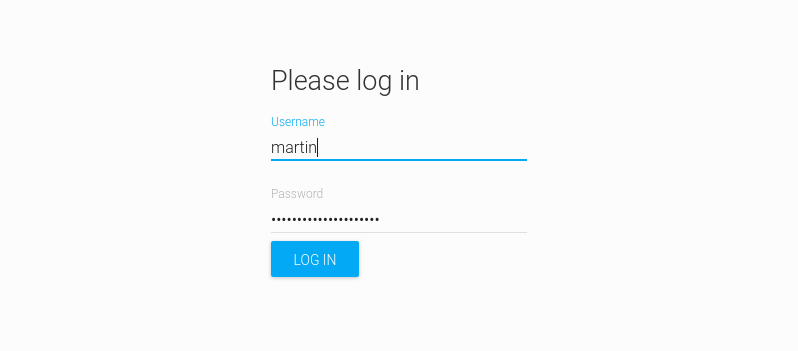
\includegraphics[width=0.8\textwidth]{img/prev-login.png}}
%	\caption{Přihlašovací formulář}
%	\label{fig:prev:login}
%\end{figure}

Po přihlášení uživatel hned vidí přehled všech meteostanic, jejich poslední záznam a má také možnost novou meteostanici vytvořit (obr. \ref{fig:app:homepage}). Jak je vidět, tak při vytváření nové meteostanice lze zadat pouze její název, nikoliv typ. Jak bylo vysvětleno v~dřívějších kapitolách, tak samotná aplikace nijak nepotřebuje řešit typ meteostanic. Převod dat do jednotného formátu je vyřešen pomocí konkretizačních členů. Po vytvoření stanice uživatel získá nové ID meteostanice, tím i způsob, jak přes GraphQL API zasílat nová data.

\begin{figure}[h]
	\centering
	\makebox[\textwidth]{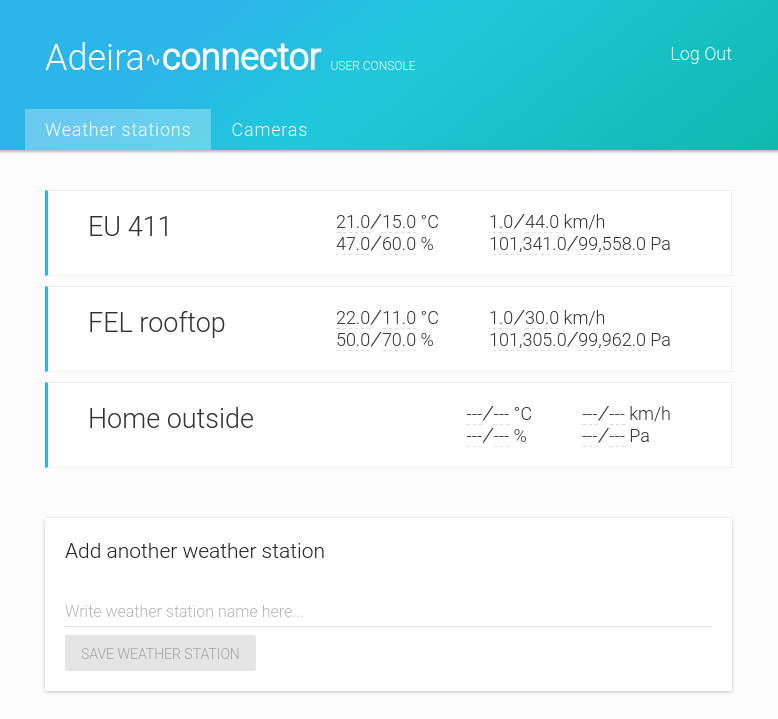
\includegraphics[width=0.8\textwidth]{img/app-homepage.png}}
	\caption{Úvodní stránka klientské aplikace}
	\label{fig:app:homepage}
\end{figure}

Vybráním jedné stanice je hned vidět její podrobný přehled. Zde je mimo jiné možné nahlédnout do historie naměřených záznamů od určitého data s~možností výběru typu agregace dat. Záznamů totiž může být velmi mnoho, proto se na serveru počítají agregované přehledy. Data je možná prohlížet si s~přesností na hodiny, popř. zvětšit časový rámec a data sdružovat po dnech, víkendech a měsících. Tak se lze teoreticky podívat na posledních 100 měsíců (pokud jsou data k~dispozici) v~rámci jednoho grafu.

Kromě výběru počátečního data a typu agregace dat je také možné zvolit způsob interpolace bodů grafů. Body lze prokládat lineární křivkou, kubickými interpolacemi, případně krokovou (skokovou) interpolací s~bodem uprostřed roviny. Záleží pak na uživateli, jaká interpolace mu vyhovuje nejvíce (obrázek \ref{fig:app:interpolation}).

\begin{figure}[h]
	\centering
	\makebox[\textwidth]{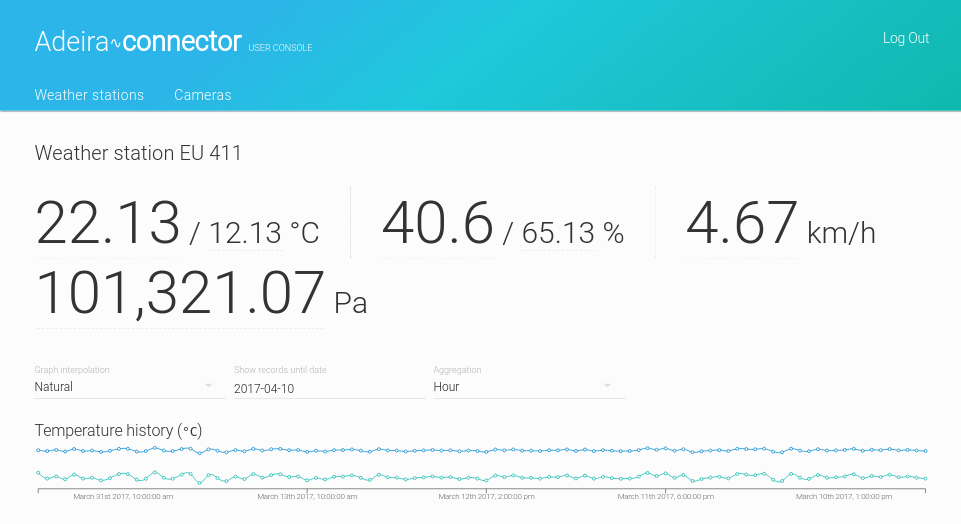
\includegraphics[width=\textwidth]{img/app-ws-detail.png}}
	\caption{Detail meteorologické stanice v~aplikaci}
	\label{fig:app:wsDetail}
\end{figure}

\begin{figure}[h]
	\centering
	\makebox[\textwidth]{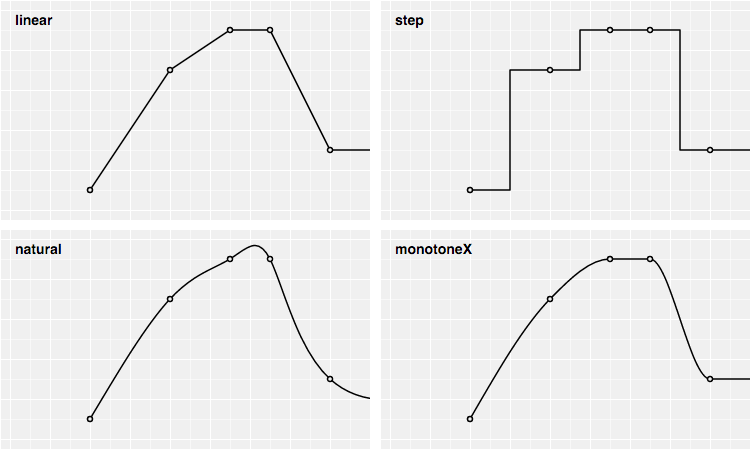
\includegraphics[width=\textwidth]{img/interp.png}}
	\caption{Způsoby interpolace grafů}
	\small zdroj: \url{https://github.com/d3/d3-shape}
	\label{fig:app:interpolation}
\end{figure}

Přehled všech IP kamer je podobný jako u~meteostanic. Zde je možné kameru přidat, přehrávat její stream a kameru zase odebrat. Prakticky se jedná pouze o~seznam video přehrávačů (viz obr. \ref{fig:app:cameras}), kdy každý přehrávač umí přehrávat vytvořený HLS stream. Popis tohoto streamu a jeho převedení z~důvodního formátu IP kamery je popsán v~dřívějších kapitolách.

\begin{figure}[h]
	\centering
	\makebox[\textwidth]{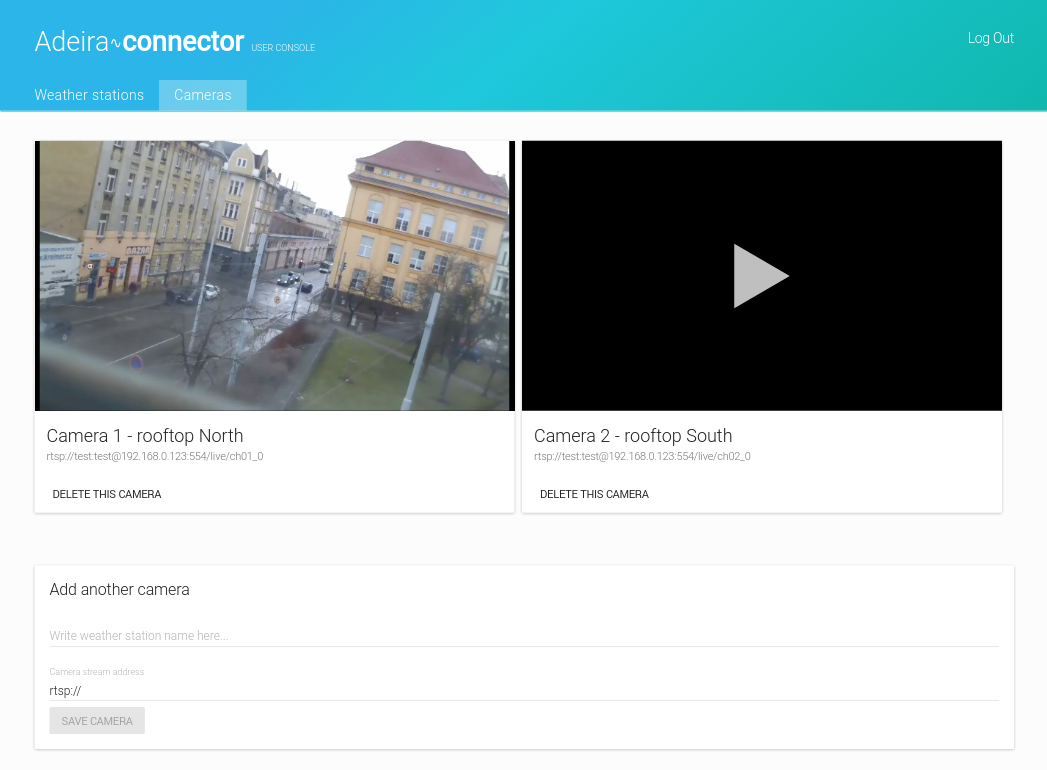
\includegraphics[width=\textwidth]{img/app-cameras.png}}
	\caption{Přehled všech video streamů v~aplikaci}
	\label{fig:app:cameras}
\end{figure}

Celé toto uživatelské prostředí funguje díky spojení Reactu a Reduxu. K~načtení aplikace dojde pouze při prvním otevření stránky a následně všechny aktualizace dat probíhají bez viditelného a obtěžujícího obnovení celé strán\-ky. Jedno z~možných vylepšení by bylo renderovat načítanou stránku na serveru. Uživatel by tak získal hotovou stránku včetně naplněného Redux úložiště. Každý další požadavek by byl obsloužen přes API stejně, jako je tomu teď. Výhoda by byla v~rychlejším prvním načtení stránky. Renderování na straně serveru je nutné také v~okamžiku, pokud budou webovou stránku indexovat webové vyhledávače. To ale není případ této administrace, která je schována za přihlášením.

%%%%%%%%%%%%%%%%%%%%%%%%%%%%%%%%%%%%%%%%%%%%%%%%%%

\section{Doporučená infrastruktura}
Na začátku této práce jsem měl veškeré potřebné nástroje pro vývoj nainstalované na svém vlastní počítači. V~průběhu vývoje jsem však postupně přešel s~celým PHP, databázemi i webovými servery do prostředí Dockeru \cite{docker} a ze svého počítače PHP odinstaloval. Rozdíl je v~tom, že dříve bylo nutné veškerý software obstarávat na jednom PC. Nově však stačí mít nainstalovaný Docker, který se chová jako velmi tenká virtualizační vrstva. Takto lze při vývoji zapnout na svém PC několik virtuálních serverů. Díky tomu je možné pohodlně využívat různé databáze nebo dokonce několik různých verzí PHP. Velký přínos je v~tom, že tyto virtuální stroje jsou jasně definovány a mohou mít naprosto stejnou podobu, jakou má produkční prostředí. Toho by se s~jedním PC dosáhlo těžko.

\begin{figure}[h]
	\centering
	\makebox[\textwidth]{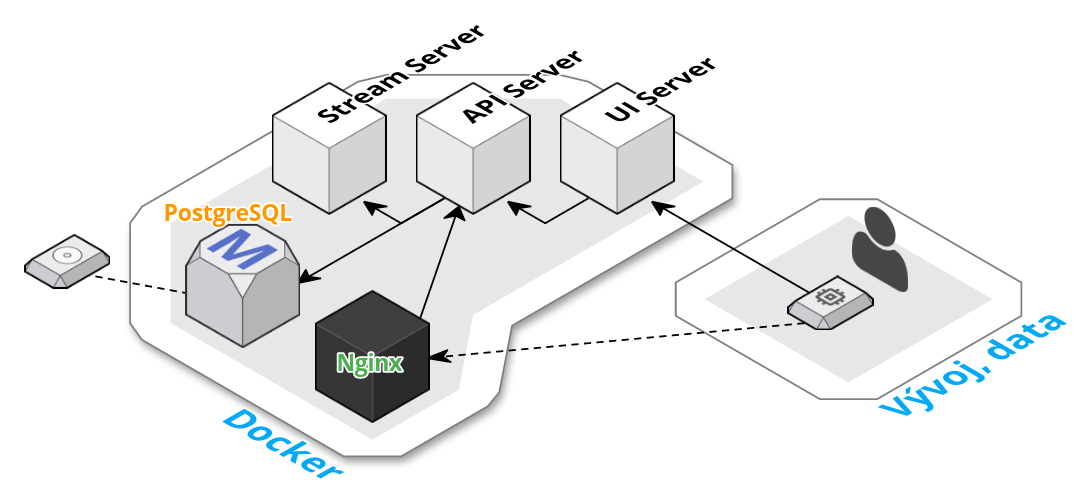
\includegraphics[width=\textwidth]{img/vyvoj-infrastruktura-crop.png}}
	\caption{Infrastruktura použitá při vývoji}
	\small zdroj: Vlastní tvorba - \url{https://cloudcraft.co/}
	\label{fig:infrastructureDevelopment}
\end{figure}

Docker se nechová jako běžně známé virtualizační platformy. Je totiž běžné, že si virtuální stroj alokuje potřebné prostředky a stroj, na kterém běží, tak velmi vytíží. Docker však využívá prostředky mnohem hospodárněji. Takže zatímco běžných virtuálních strojů je možné zapnout jednotky až desítky, tak tzv. Docker kontejnerů je možné spustit stovky až tisíce na jednom počítači. A~to už by byla hodně velká infrastruktura - rozhodně dostatečná pro potřeby této aplikace. Na obrázku \ref{fig:infrastructureDevelopment} je znázorněno Docker prostředí, které je pro tuto aplikaci vhodné.

Jak je možné, že Docker zvládne tak velké množství virtálních strojů? Docker může používat více souborových systémů, ale takovým hlavním zá\-stup\-cem je AUFS \cite{aufs}. AUFS je vrstvený souborový systém, jehož hlavní předností je možnost mít sdílené vrstvy operačního systému pouze pro čtení a individuální tenké vrstvy s~možností zápisu, které obsahují odlišnosti jednotlivých strojů. Pokud tedy server sdílí společnou část svého systému s~jiným serverem, tak si nenárokuje dodatečné prostředky, ale sdílí je. Servery zároveň nemohou nijak kolidovat, protože spodní vrstvy souborového systému jsou pouze pro čtení. Sdílení prostředků není jediný přínos. Nastartování nového serveru v~rámci Dockeru trvá zhruba jednu sekundu (mnohdy ani to ne)\footnote{Záleží na tom, co se v~kontejneru startuje za procesy. Doporučený postup je však držet kontejnery co nejméně náročné a starající se o~jednu věc.}. Je tedy možné spustit proces z~příkazové řádky, ale ve skutečnosti spustit celý Docker kontejner a proces spustit izolovaně v~kontejneru. Díky extrémní rychlosti startování je to téměř neznatelná změna.

Ale zpět ke vhodné infrastruktuře. Doposud popisované řešení pomocí Dockeru není jediné možné. Pokud by to bylo nutné, může aplikace fungovat pouze na jednom serveru. Je totiž potřeba pouze webový server, který bude přijímat HTTP požadavky a směřovat je na PHP. Dále je potřeba PostgreSQL databáze a to je vlastně vše. Webové rozhraní může být zatím vybavováno jako statická stránka (neprobíhá renderování na serveru), takže nepotřebuje žádné zvláštní služby. Stejně tak streamovací server pro zpracovávání videa potřebuje pouze PHP. Je však vhodné oddělit jednotlivé závislosti, aby bylo možné škálovat aplikaci nezávisle podle potřeby. Na to se opět perfektně hodí Docker, kde je běžné mít jeden běžící proces v~jednom kontejneru (nebo alespoň jeden druh procesu). Proto má webový server i PHP vlastní kontejnery.

Vývojové prostředí může být zcela totožné s~produkčním prostředím, ale nemusí tomu tak být. Na produkci je často potřeba dalších služeb, které různým způsobem optimalizují běh aplikace např. pro vysokou zátěž (CDN, vyvažování zátěže, replikace databází). Tento stav je znázorněn na obrázku \ref{fig:infrastructure}.

\begin{figure}[h]
	\centering
	\makebox[\textwidth]{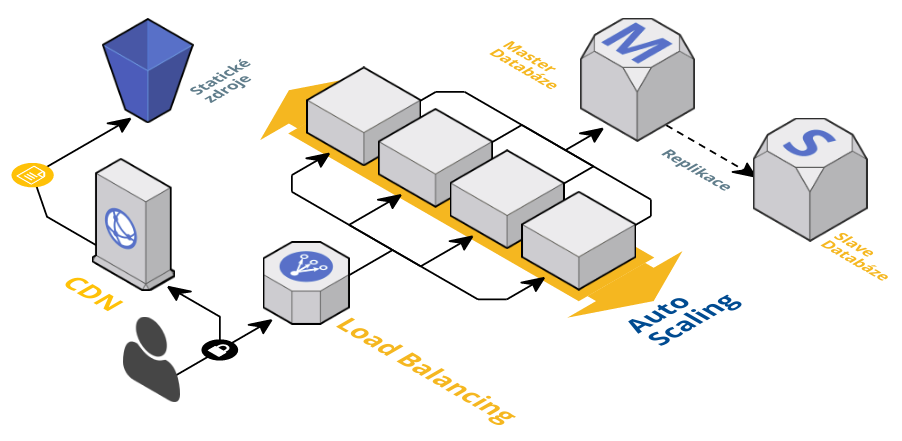
\includegraphics[width=\textwidth]{img/doporucena-infrastruktura-crop.png}}
	\caption{Doporučená infrastruktura}
	\small zdroj: Vlastní tvorba - \url{https://cloudcraft.co/}
	\label{fig:infrastructure}
\end{figure}

Takové rozložení strojů je jednoznačně násobně dražší než provoz na jednom serveru. Při rozhodování se o~infrastruktuře je nutné dobře propočítat a rozhodnout se, jak velká investice dává smysl. Pokud bych se rozhodl tuto aplikaci provozovat jako službu zákazníkům, tak by bylo nutné se k~něčemu podobnému přibližovat. Pro soukromé účely by naopak stačil nějaký obyčejný sdílený hosting.

%%%%%%%%%%%%%%%%%%%%%%%%%%%%%%%%%%%%%%%%%%%%%%%%%%

\section{Možnosti rozšíření díky API}
Na začátku programování hlavní aplikace nebylo úplně jasné, jak vše dopadne. V~současné době jsem však přesvědčen, že vytvoření uzavřené aplikace s~API bylo jednoznačně správné řešení. Aplikace se stará \textbf{jen} o~ukládání a vybavování dat, popř. o~autorizaci. Díky tomu je možné soustředit se na to, aby vše fungovalo co nejlépe. Není třeba řešit velké množství různorodých meteostanic. Aplikace vlastně rozumí libovolné meteostanici, protože ona odesílá do API data a ta už mají jednotný formát.

Klíčové je využití GraphQL, které nevytváří statické koncové výstupy, ale umožňuje získávat z~API libovolná data. Příkladem využití API mohou být exporty dat. Bylo by možné vytvořit další funkcionalitu a data umožnit exportovat. Ale to nebylo cílem. Server se stará o~API. A~když existuje grafové API, tak je možné data také exportovat. Například následující GraphQL dotaz vrátí všechny kamery, meteostanice a~jejich data:

\begin{minted}{graphql}
{
  allCameras {
    id, name, stream { source, hls }
  }
  allWeatherStations {
    totalCount, weatherStations {
      id, name, allRecords(first: 10) {
        totalCount, returnedCount, records {
          aggregatedDate, absolutePressure, relativePressure
          indoorTemperature, outdoorTemperature,
          indoorHumidity, outdoorHumidity, windSpeed,
          windAzimuth, windGust
        }
      }
    }
  }
}
\end{minted}

Ze serveru se vrátí JSON odpověď, která je velká několik MB a obsahuje všechny potřebné informace. Není nutné mít předem definovanou strukturu odpovědi. Pouze pokud by bylo třeba exportovat data např. ve formátu XML a mít export velmi rychlý, vyplatí se tuto funkcionalitu dodělat.

Na rozdíl od jiných běžných API je GraphQL (jak název napovídá) grafové. Je nutné dotazovat se na konkrétní cestu v~grafu a tato data se vrátí. Neexistuje tedy pevná struktura odpovědi a to je jeden z~důvodů, proč toto API není třeba verzovat \cite{graphql:versioning}. Nové vlastnosti lze jednoduše přidat a zastaralé lze schovat (i když budou dále fungovat). Prakticky tedy neexistuje nic jako jedna verze API. API může být každý den jiné, ale vždy zpětně kompatibilní - podobně jako je nutné dělat změny v~rámci databázových migrací.

Myšlenka grafového API je natolik mocná, že se dnes začíná GraphQL používat jako proxy pro jiná (starší) API. Funguje to tak, že klienti posílají dotazy na GraphQL a toto API pouze překládá požadavky na např. REST API, které má pevnou strukturu. Tak lze získat všechny vlastnosti GraphQL i zpětně. Není pak složité postupně začít staré API odstraňovat. API lze tedy libovolně rozšiřovat díky jednotnému rozhraní, které je připraveno pro neustálé změny.